% 四阶龙格库塔法

\pentry{中点法解常微分方程(组)\upref{OdeMid}}

\bb{龙格库塔法} 是一类数值解微分方程的算法, 其中较常见的是\bb{四阶龙格库塔法}. 这里不进行推导, 仅仅给出公式如下($y_n, t_n, h$ 的定义类比\autoref{OdeNum_eq5}\upref{OdeNum})
\begin{equation}\label{OdeRK4_eq1}
y_{n+1} = y_n + \frac h6 (k_1 + 2k_2 + 2k_3 + k_4)
\end{equation}
其中
\begin{equation}\label{OdeRK4_eq2}
\ali{
k_1 &= f(y_n, t_n) 
& k_2 &= f \qty(y_n + h\frac{k_1}{2}, t_n + \frac h2 )\\
k_3 &= f \qty( y_n + h\frac{k_2}{2}, t_n + \frac h2 ) \qquad
&k_4 &= f(y_n + hk_3, t_n + h)
}\end{equation}
由以上两式, 不难把该算法拓展到方程组的情况. 对于 $N$ 元微分方程组
\begin{equation}\leftgroup{
y'_1(t) &= f_1(y_1,\dots, y_N, t)\\
y'_2(t) &= f_2(y_1,\dots, y_N, t)\\
& \vdots\\
y'_N(t) &= f_N(y_1,\dots, y_N, t)
}\end{equation}
我们可以把该式记为矢量函数的形式
\begin{equation}\label{OdeRK4_eq4}
\vec y'(t) = \vec f(\vec y, t)
\end{equation}
现在我们仅需要把\autoref{OdeRK4_eq1} 和 \autoref{OdeRK4_eq2} 中的所有 $y_i$ 和 $k_i$ 都变为 $N$ 维列矢量 $\vec y_i$ 和 $\vec k_i$ 即可将微分方程拓展为微分方程组.

\subsection{例程}

到目前为止, 我们每求一个微分方程的数值解都要重新写一次程序, 对于一些较为复杂的算法这样做效率较低. 我们这里不妨把四阶龙格库塔法写到一个单独的函数文件 odeRK4.m 中, 当我们要解某个特定的方程时, 只需把\autoref{OdeRK4_eq2} 中的 $f(y, t)$ 作为自变量输入即可解出 $y(t)$.

\Code{odeRK4}

我们先来看第 1 行的函数声明, 输入变量中,\x{f} 是\autoref{OdeRK4_eq4} 中 $\vec f(\vec y, t)$ 的函数句柄\upref{MatFun}, \x{tspan} 是一个 \x{2×1} 的列矢量, \x{tspan(1)} 是初始时间, \x{tspan(2)} 是终止时间, \x{Y0} 是一个列矢量, \x{Y0(ii)} 是第 \x{ii} 个因变量的初始值, \x{Nt} 是 $t_n$ 的个数, \x{tspan} 定义的时间区间被等分为 \x{Nt - 1} 个小区间. 因变量中, \x{Y} 的行数是因变量的个数, 列数是 \x{Nt}, \x{t} 是一个行矢量, 由第 6 行定义, \x{Y(ii, jj)} 就是第 \x{ii} 个变量在 \x{t(jj)} 时刻的值. 第 5 行把初值 \x{Y0} 赋给 \x{Y} 的第 1 列, 第 8-14 行的循环根据\autoref{OdeRK4_eq1} 和\autoref{OdeRK4_eq2} 的矢量形式由 \x{Y} 的第 \x{ii} 列($\vec y_i$)求第 \x{ii+1} 列($\vec y_{i+1}$).

我们先来用这个函数来计算“天体运动的简单数值计算\upref{KPNum0}” 中的问题. 我们令因变量 $\vec y$ 的四个分量依次为一阶方程组(\autoref{OdeNum_eq4}\upref{OdeNum})
\begin{equation}\label{OdeRK4_eq5}
\leftgroup{
x' &= v_x\\
y' &= v_y\\
v'_x &= -GMx/(x^2 + y^2)^{3/2}\\
v'_y &= -GMy/(x^2 + y^2)^{3/2}
}\end{equation}
中的 $x, y, v_x, v_y$. 程序代码如下

\Code{keplerRK4}

运行结果如\autoref{OdeRK4_fig1} 所示.

\begin{figure}[ht]
\centering
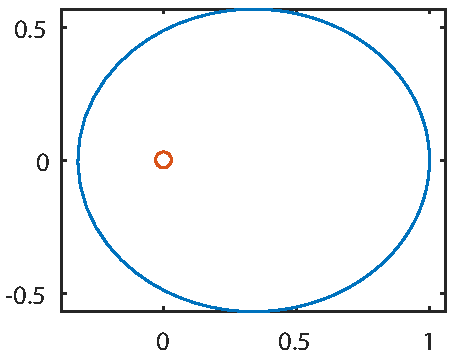
\includegraphics[width=7cm]{./figures/OdeRK41.pdf}
\caption{运行结果} \label{OdeRK4_fig1}
\end{figure}

我们先来看函数 \x{fun} (20 行), 这个函数就相当于\autoref{OdeRK4_eq5}. 第一个输入变量 \x{Y} 是一个列矢量, 是 $\vec y_n$ 的值, 第二个输入变量是 $t$, 但由于\autoref{OdeRK4_eq5} 中没有出现 $t$, 我们用波浪线代替. 第三个输入变量是参数 $GM$, 即万有引力常数和中心天体质量之积. 输出变量 \x{Y1} 是一个列矢量, 是 $\vec y'_n$ 的值.

再来看主函数 \x{KeplerRK4} (第 1 行), 参数设定中除了步数从 4000 变为了 100, 其他都和“天体运动的简单数值计算\upref{KPNum0}” 中的程序一样, 然而这里运行结果却精确得多(曲线几乎闭合), 可见这种算法的优越性.

主函数第 10 行中将 \x{fun(Y, t, GM)} 变为函数句柄 \x{f(Y, t)}, 这样 \x{GM} 就可以在“参数设定” 中设置, 而不用在 \x{fun} 函数内部设置. 第 11 行调用了上文中的 \x{odeRK4} 函数解方程组, 由于我们在画图时不需要用 \x{t}, 所以把第二个输出变量改为波浪线.
